\documentclass[aspectratio=169]{beamer}

\usepackage[utf8]{inputenc}
\usepackage[english]{babel}
\usepackage[T1]{fontenc}
\usepackage{graphics}

\setbeamertemplate{navigation symbols}{}
\usetheme{CambridgeUS}
\usecolortheme{dolphin}


\author[MABILEAU, STAUFFER]{
    Paul MABILEAU
    \and
    Franck STAUFFER
    \and
    \texttt{\{paul.mabileau,franck.stauffer\}@telecom-sudparis.eu}
}
\institute[TSP]{TELECOM SudParis}

\title[RINA's security]{Recursive Inter-Network Architecture's Security}
\subtitle{Security of an IPC network}
\subject{Network paradigm}

\logo{
\includegraphics[width=1cm]{img/tsp.png}}
\date[2020/05/27]{May 27, 2020}

\AtBeginSection[]{\frame{\sectionpage}}
\setcounter{tocdepth}{1}


\begin{document}
\maketitle

\begin{frame}
    \frametitle{Forecast}
    \begin{itemize}
        \item Networking is only Inter-Process Communication (IPC)
        \item Current `internet' is not an actual inter-network
        \item Networking can be much more simple
    \end{itemize}
\end{frame}

\frame{\frametitle{Table of contents}\tableofcontents}


\section{Introduction}

\subsection{Motivation}
\begin{frame}
    \begin{itemize}
        \item TCP/IP is old
        \item TCP/IP is complex
        \item TCP/IP is not adapted to modern issues
    \end{itemize}
\end{frame}

\subsection{Problem Statement}
\frame{\centering Is RINA a secure alternative to TCP/IP?}


\section{RINA architecture}

\subsection{IPC Process}
\frame{\centering
\includegraphics[scale=2]{img/IPCP.png}}
\subsection{IPC API}
\frame{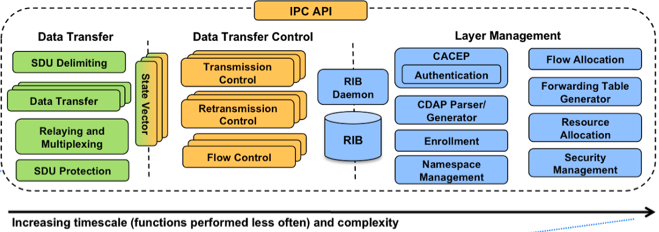
\includegraphics[width=\textwidth]{img/API.png}}
\subsection{Ditributed IPC Facility}
\frame{
\includegraphics[width=\textwidth]{img/DIF.png}}
\subsection{Layers}
\frame{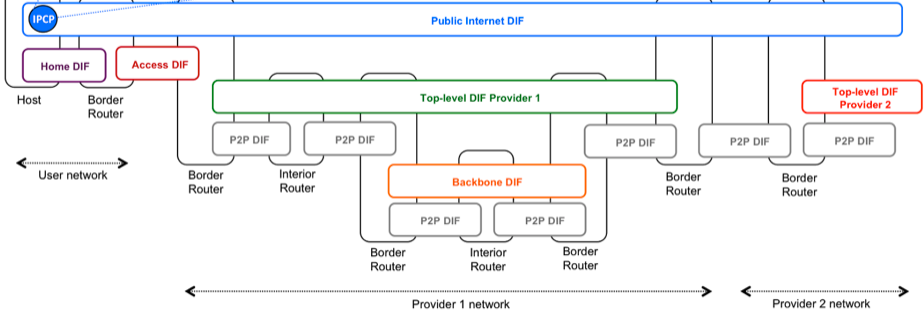
\includegraphics[width=\textwidth]{img/layers.png}}
\subsection{Distributed Application Process}
\frame{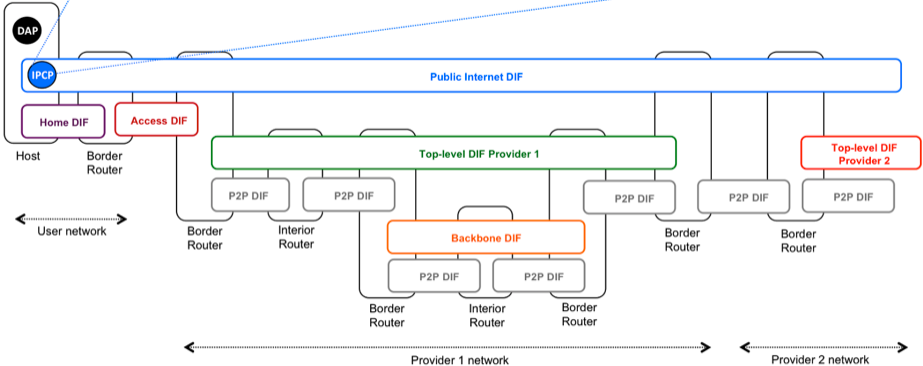
\includegraphics[width=\textwidth]{img/DAP.png}}
\subsection{Distributed Application Facility}
\frame{\centering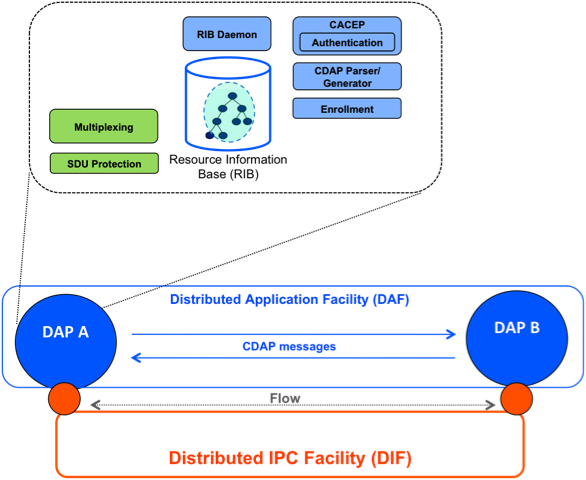
\includegraphics[height=\textheight]{img/DAF.png}}


\section{Conclusion}
\end{document}

